\documentclass[12pt, a4paper, titlepage]{article}

% VARIABLES
% Change these to suit your essay.
\def\thetitle{SDP Group Report - Milestone 2}
\def\theauthor{Group 4}

% FONTS
\usepackage{fontspec} 
\usepackage{xunicode}
\usepackage{xltxtra}
\defaultfontfeatures{Mapping=tex-text}
\setromanfont[Ligatures={Common},
	BoldFont={Adobe Garamond Pro Bold},
	ItalicFont={Adobe Garamond Pro Italic}]{Adobe Garamond Pro}
\setmonofont[Scale=0.8]{Monaco} 

% DOCUMENT LAYOUT
\usepackage{geometry} 
% Change this if you have specific margins to use.
\geometry{a4paper, left=0.8in, right=0.8in}

% HEADERS
\usepackage{fancyhdr}
\pagestyle{fancyplain}
\rhead{\textsc{\theauthor}}
\lhead{\textsc{SDP Group Report - Milestone 1}}
\setlength{\headheight}{14.5pt}

% HEADINGS
\usepackage{sectsty} 
\usepackage[normalem]{ulem} 
\sectionfont{\rmfamily\bfseries\upshape\Large}
\subsectionfont{\rmfamily\bfseries\upshape\normalsize} 
\subsubsectionfont{\rmfamily\mdseries\upshape\normalsize} 

\usepackage{titlesec}
\titleformat{\section}{\large\bfseries\raggedright}{}{0em}{\thesection\hspace{1em}}[\titlerule]

% SYMBOLS & MATHS
\usepackage{amsmath}
\usepackage{marvosym}
\usepackage{url}

% SOURCE CODE
\usepackage{minted}

% TODOs
\usepackage{todonotes}

% GRAPHICS
\usepackage{titlepic}
\usepackage{graphicx}

% PDF SETUP
\usepackage[dvipdfm,bookmarks,colorlinks,breaklinks,pdftitle={\thetitle},pdfauthor={\theauthor}]{hyperref}  
\hypersetup{linkcolor=black,citecolor=black,filecolor=black,urlcolor=blue} 

% TITLE PAGE
\setlength{\headsep}{5mm}

\title{\small{SDP Group Report - Milestone 1} \\ \huge Group 4 -- Castle Crashers}
\author{Andrew Johnstone \and Callum Stott \and Christopher Brown \and Daniel Wren \and Emil Georgiev \and Katherine Findlay \and Magdelena Konkiewicz \and Sittikorn Assavanives \and Steven Skelton \and William Bradshaw}
\date{\today}
\titlepic{
\includegraphics[width=0.8\textwidth]{images/team-logo.png}\\[1cm]}

\begin{document}
\maketitle

\section{Introduction}

During the third and fourth week of the System Design Project (SDP) our team
worked steadily towards the goals we set in our first report. Throughout this
report we will be discussing how we achieved these goals and what tasks were
undertaken throughout the two weeks up to the second milestone.

\section{Programming}

Large improvements and milestones were made and met in the programming tasks.
The system was fully integrated, the vision improved, the testing expanded and
the strategy enhanced.

\subsection{Integration}

System integration was going to be a key problem for this milestone and for
the project as a whole. Since our system design specifies that the vision
and the strategy are split up, the integration of these two systems are
key to our success. Originally we were going to have the vision server and
the client in the strategy communicate by sending JSON (Javascript Object
Notation) that described the world state between them. This was not used
because it was unnecessarily difficult to create a protocol and make both
sides use it properly. To combat this we decided to use Google Protocol
Buffers\cite{protobuf}. This allowed us to create a protocol and then generate
files that adhere to it. This allowed the vision and strategy systems to be
developed in almost complete isolation, each knowing that the other would stick
to its side of the contract in the protocol.

\subsection{Vision}

Our aims for the vision system included accurately tracking the position and
orientation of each of the objects visible on the pitch. Also making the
positions and orientations available for use by the robot’s, independently
running, control and strategy systems.To successfully achieve our first goal of
tracking positions and orientations of objects we built on the progress of the
vision system from the last milestone. Tracking the positions of the objects
involved converting the input image from the camera to the hue saturation value
(HSV) colour space and creating binary images by isolating the red ball, the
yellow or blue crosses. The center of mass of the binary images can then be
calculated and will give the correct position of each object. Our first attempt
at calculating orientations was to isolate the black circles. Once they had been
found, the circle center point and the center of mass of the object could be
used in the following formula to determine the orientation of the robot:
\begin{equation*}
\mbox{Orientation} = (\arctan2(\mbox{circleCenter}, \mbox{crossCenter}) \times \left(\frac{180}{\pi}\right) + 450) \mod 360
\end{equation*}
After several tests with the cross plates on the robots we decided that this
method was not accurate enough. As the colour being searched for was black, it
was too difficult to isolate from shadows and our own robot. This difficulty
meant that the angle calculated would vary wildly and was often incorrect. To
temporarily remedy the situation, the engineering team added two white blocks
to the top of our robot which were much easier to isolate and were used to
calculate the orientation using the same formula.

\subsection{Strategy}

For this milestone we implemented a simple strategy for navigating to the ball
which calculated a vector between our robot and the ball and drives along it.
This allowed us to use our current control framework directly to turn the robot
the required amount and then drive until it reached the ball. Additional work
was done on a more advanced strategy that utilizes an A* search algorithm to
calculate the best cost path to the ball. However, as this is a more complex
implementation it wasn’t ready for the milestone so we opted to use our
simpler strategy for the demonstrations.

The beginning of a strategy framework was added during the work for this
milestone. It is the start of some work that makes strategy code easier to
write and test. Multiple strategies can be compared against one another in
the simulator and compared as to their effectiveness. Other benefits of using
the framework is that new strategies are easy to test, tweak and maintain. In
general the system increased modularity and will allow many people to work on
improving strategies without stepping on each other’s toes.

\subsection{Simulator}

It became clear that, with the amount of work we’d have to do on strategy,
we needed a way to test it. For this we started implementing a simulator. Our
initial simulator was just a visual representation of the world state object
used by the strategy component. To integrate it for testing the strategy we have
been developing it share a world state with the strategy that the simulator
can alter. We have been accomplishing this by using an extension of our robot
control abstraction to send commands to the simulator rather than to a robot.
This is another feature which we did not complete for this milestone but is to
become one of our key goals during development for milestone three.

\subsection{Testing}

Testing the project has made large improvements from the first milestone. The
system is now using unit tests to test all of the key aspects of the system. For
the next milestone we are planning on extending these unit tests further and
adding integration tests to aspects of our strategy before working with the new
simulator to test the system as a whole and to see if our strategies achieve
their high level goals.

\subsection{Development Process}

Since the beginning of the project we were eager to make sure that we didn't
hold back development with inefficient processes and lack of communication.
We have been using Git\cite{git-scm} as our version control system and its
simple branch mechanism allows us to easily work on features without stepping
on others toes. We initially had a work flow that consisted of a master branch
and a branch for individual features but the code soon became too complex. We
reassessed and now have a development and a master branch and merge features
into develop. This is based on a popular archetypal git workflow. So far we
only merge into development into master after a milestone. Another example of
our development process is our use of tools such as Campfire\cite{campfire} -
a persistant instant messaging web application. This allows us to remain in
constant contact with the rest of our team while also providing a method for
quick fire collaboration with others. Issues are entered into an issue tracker
for the rest of the team to see and fix.

\subsection{Future Plans}

Our future plans include full simulator integration to add to an already
expanding test suite. In addition to testing, other code quality improvements
such as adding to our internal wiki and completing code documentation. The
vision code will be improved to use a more reliable method of finding the
angles of the robots. All of the remaining time will be taken up with writing
strategies that allow us to complete the next objective and on to the first
match.

\section{Engineering \& Construction}

\subsection{Goals}

Our goals are to produce a robot that drives fast, kicks hard, dribbles the ball
efficiently, and performs off-the-wall kick. Additionally, trying to reduce the
slippage of the tank tracks.

\subsection{Achievements}

After the first deliverable we compared our robot against the other teams. We
found that we had an average speed but had one of the most powerful kickers.
We were also the only team to implement a spinner. We decided to focus on the
kicker and spinner in order to give us maximal advantage.

\subsection{Kicker}

To improve the kicker we acquired a second NXT motor for the kicker (Figure
\ref{fig:topview}). This provided us with much more power, allowing us to gear
the kicker to increase speed. Previous gearing attempts had failed because we
had insufficient torque. After experimenting with gearing the kicker up further
we found a 5:3 gear ratio to be the most effective. This allows us to launch the
ball \_\_\_ m. Overall, we are very happy with our kicker but are exploring a
levered system in order to augment it further.

\subsection{Spinner}

In order to develop the spinner we implemented used a different style of wheels.
These new, larger wheels (Figure \ref{fig:spinner}) provide much more friction,
which increases the backspin placed on the ball. We have had this spinner
approved by Garry. The new spinner system gives us much more control. The
previous incarnation helped us to drive forward with the ball, while the new
spinner lets us dribble, reverse, and even turn while in possession of the ball.
Overall, our spinner works very well and should not need further development.

\subsection{Future Plans}

For the next milestone we will target our movement system. We shall do this
by first investigating rubber tank tracks which would provide better grip,
hopefully stopping the robot from slipping while driving. If this does not
sufficiently improve our robot we will consider changing the tank tracks to
wheels as they can provide precise turning on the spot.

It is also our intention to implement a light sensor to detect the presence of
the ball. This could help us in deciding when to kick.

\newpage

\setcounter{section}{5}
\begin{thebibliography}{9}

\bibitem{protobuf}
	Google Protocol Buffers,
	\url{http://code.google.com/apis/protocolbuffers/}

\bibitem{git-scm}
	Git Source Control Management,
	\url{http://git-scm.com}

\bibitem{campfire}
	Campfire,
	\url{http://campfirenow.com/}

\end{thebibliography}

\appendix

\section{Goals}

\section{Photographs}

\begin{figure}[h]
\begin{minipage}[b]{0.5\linewidth}
\centering
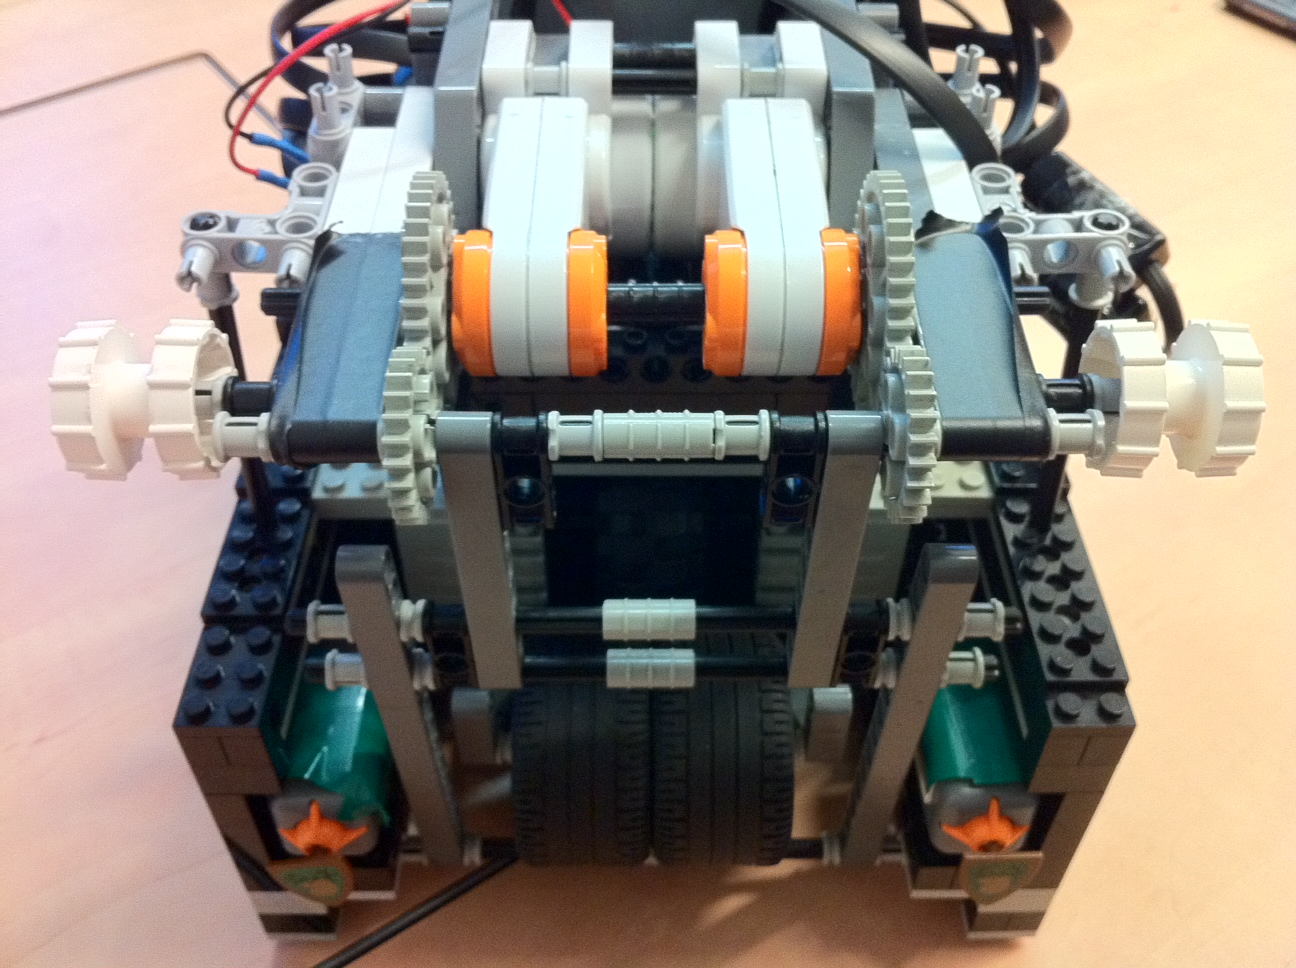
\includegraphics[scale=0.2]{images/robot/topview.jpg}
\caption{Top View}
\label{fig:topview}
\end{minipage}
\hspace{0.5cm}
\begin{minipage}[b]{0.5\linewidth}
\centering
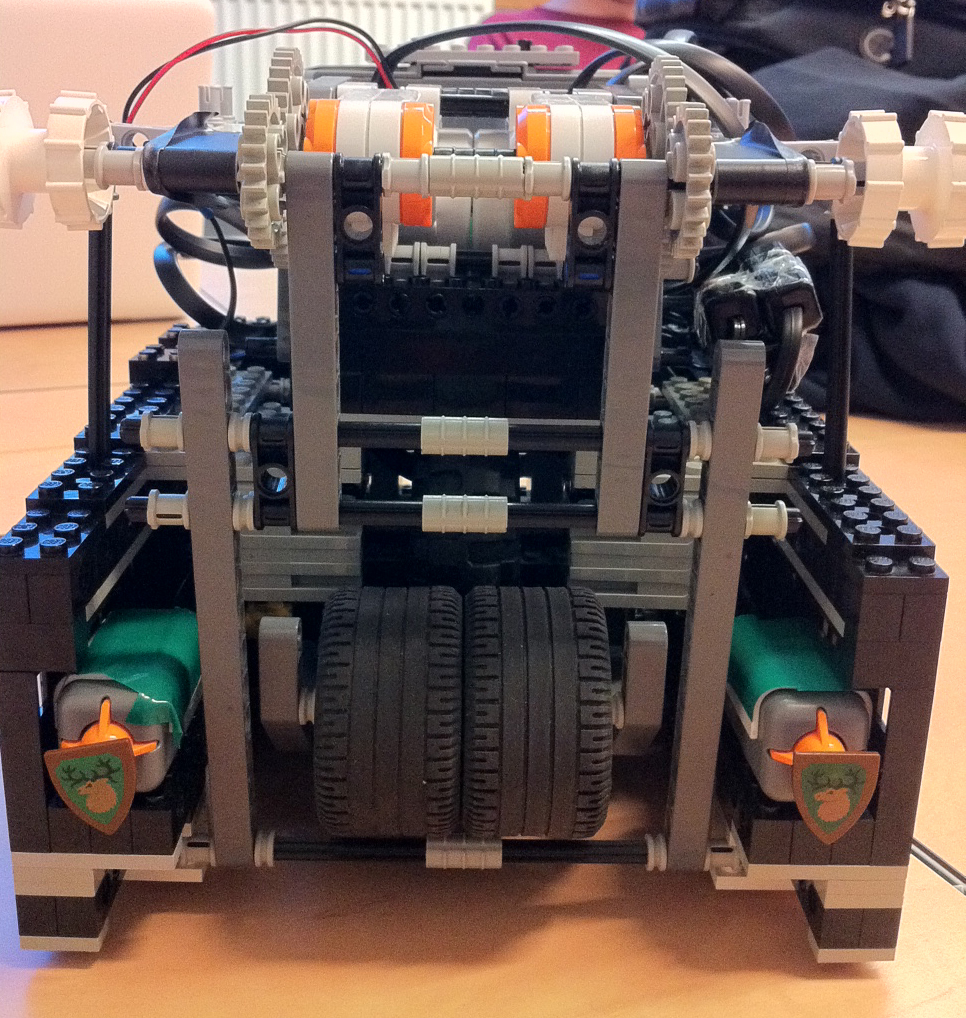
\includegraphics[scale=0.2]{images/robot/frontview.jpg}
\caption{Front View}
\label{fig:frontview}
\end{minipage}
\end{figure}

\begin{figure}[ht]
\begin{minipage}[b]{0.5\linewidth}
\centering
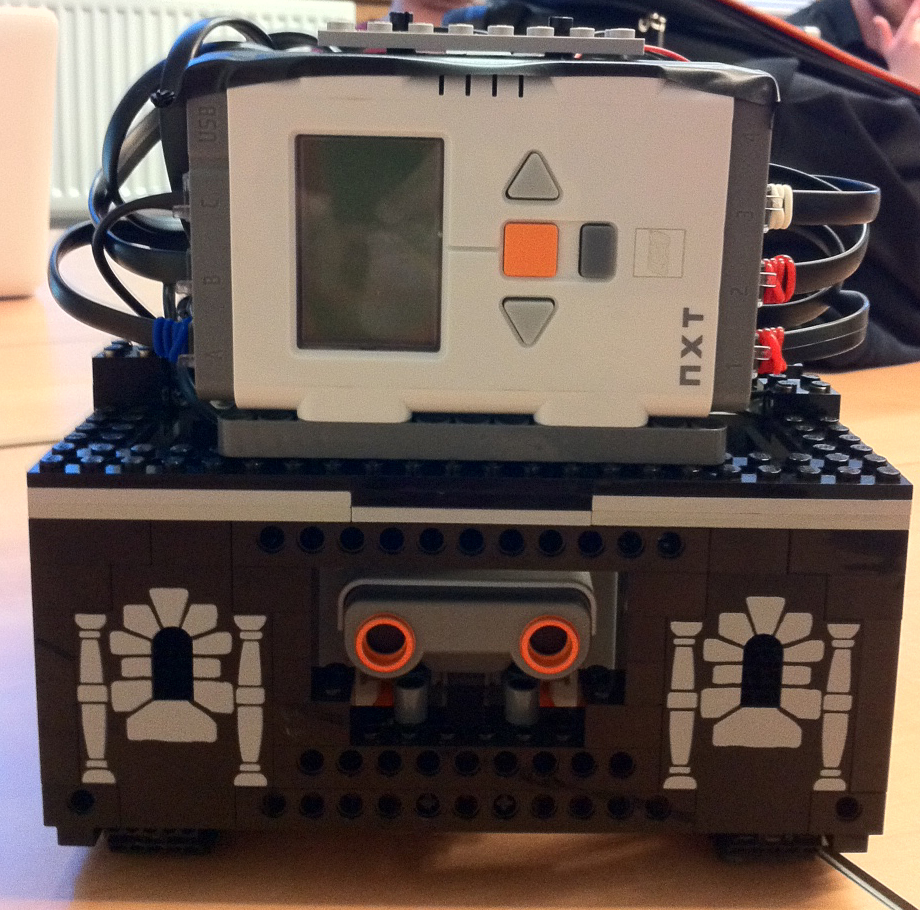
\includegraphics[scale=0.2]{images/robot/backview.jpg}
\caption{Back View}
\label{fig:backview}
\end{minipage}
\hspace{0.5cm}
\begin{minipage}[b]{0.5\linewidth}
\centering
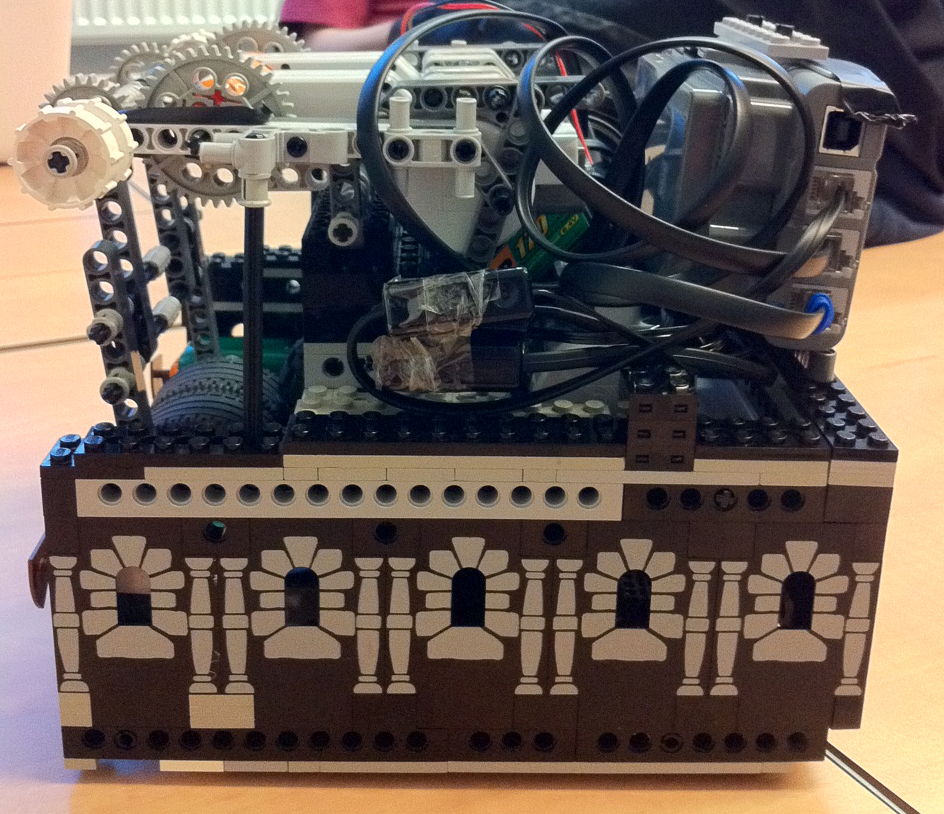
\includegraphics[scale=0.2]{images/robot/sideview.jpg}
\caption{Side View}
\label{fig:sideview}
\end{minipage}
\end{figure}

\begin{figure}[ht]
\begin{minipage}[b]{0.5\linewidth}
\centering
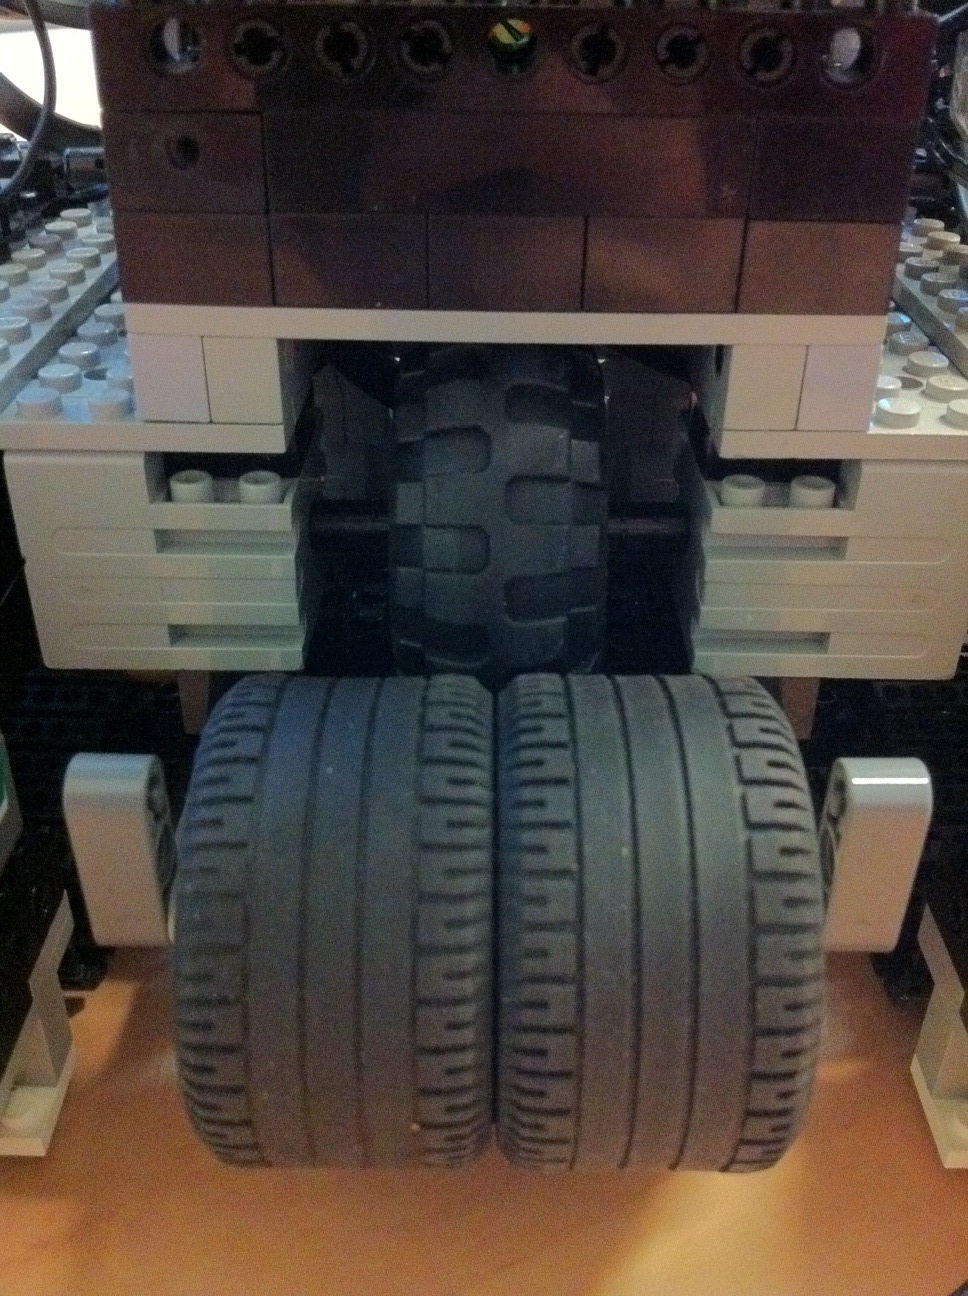
\includegraphics[scale=0.2]{images/robot/spinner.jpg}
\caption{Spinner}
\label{fig:spinner}
\end{minipage}
\hspace{0.5cm}
\begin{minipage}[b]{0.5\linewidth}
\centering
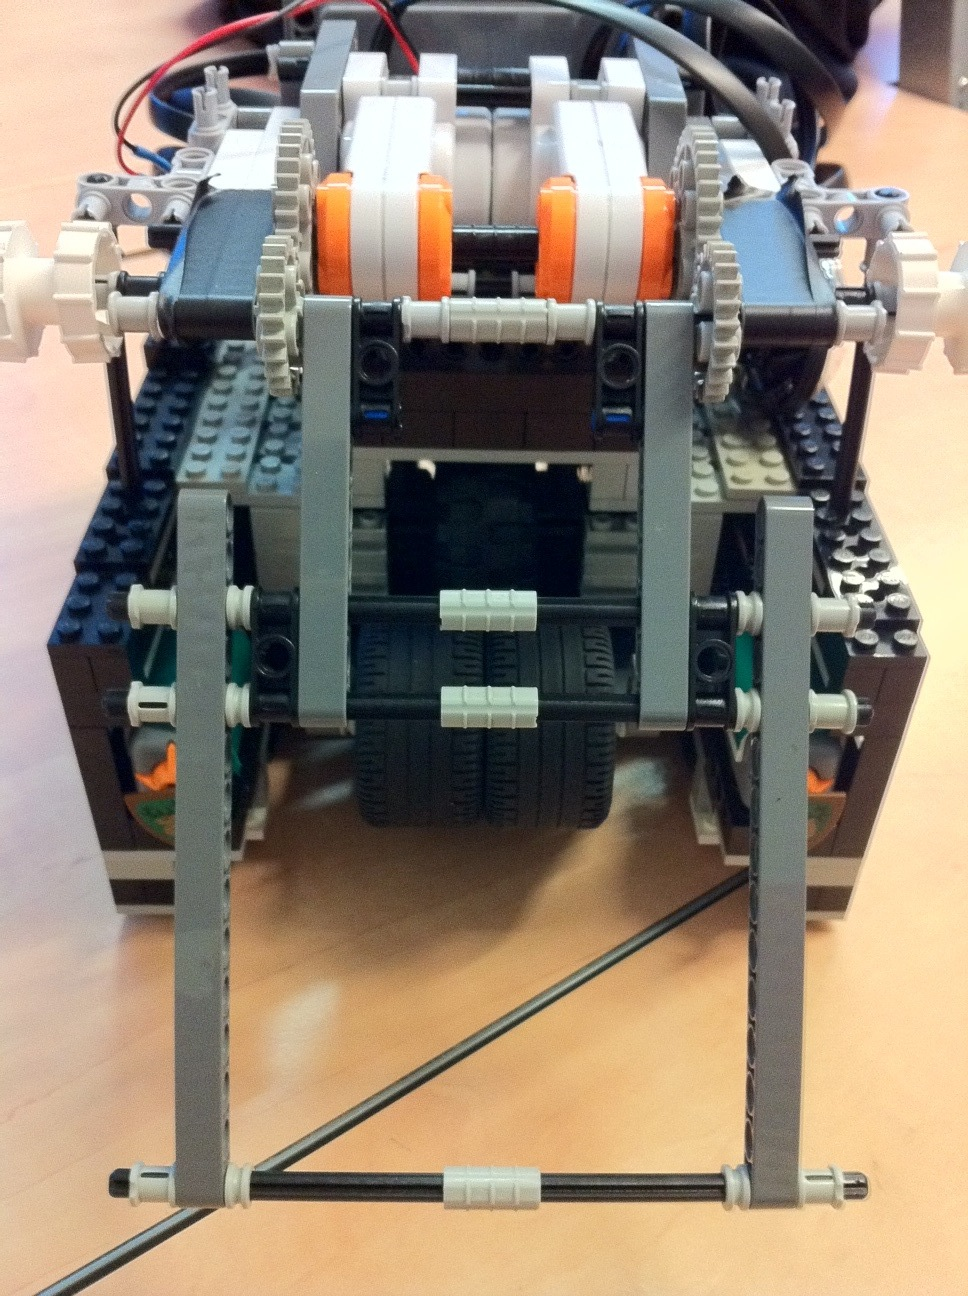
\includegraphics[scale=0.2]{images/robot/kicker.jpg}
\caption{Kicker}
\label{fig:kicker}
\end{minipage}
\end{figure}

\end{document}
